\documentclass{article}
	\usepackage{graphicx}

	\begin{document}

	\title{HW/SW Entwurfssprachen am Beispiel System-C}
	\author{Florian Zaruba, Thomas Weber}

	\maketitle

	%\begin{abstract}
	%The abstract text goes here.
	%\end{abstract}

	\section{HW/SW Design Languages}
	tba
	\section{What is SystemC}
	SystemC is a High Level Abstraction Language which aims to combine the benefits of hardware description languages and software.
	
	Hardware description languages have the big advantage that they are very performant.
	They execute exactly this operations for which they are designed for.	
	Software that runs on a processor is relatively easy to read and can be, in contrast to HDL, easy  tested and verified.	
	The long compilation process of the hardware modules and the design cycle which is very time consuming, hence the whole partitioning procedure had to be passed, make a better solution desireable.
	Futhermore hardware cannot be easily tested and verified and it cannot be updated\footnote{Except over an JTAG interface, in configureable chips like FPGAs}.
	
	SystemC shortens the design cycle because it makes it possible to write hardware and software in one language.
	It is an additional library to C/C++ which is mostly used in context of embedded systems today.
	The SystemC modules can be compiled in hardware and the C/C++ program which uses this modules fits best on the chip hence both components are tested together.
	  \subsection{History}
	    SystemC were introduced in 1999 as SystemC 1.0. At this time it provided some basic features, e.g., Signals, Simulation of a kernel and fixed point arithmetic.
	    It was also possible to break down designs it into modules in order to reuse code.
	    
	    SystemC 2.0 was started in the late 2000. It extends the previous version with events as primitive behavior triggers as well as channels, interfaces and ports.
	    It was also more powerful in modeling at transaction level.
	    Furthermore its complete library were new coded to upgrade it to an independent System Level Description Language (SLDL).
		\subsection{Copmparision}
		Several languages have emerged to address the various aspects of system design. Although Ada and Java have proven their value, C/C++ is predominately used today for embedded system software. The hardware description languages (HDLs), VHDL and Verilog, are used for simulating and synthesizing digital circuits. Vera and e are the languages of choice for functional verification of complex application-specific integrated circuits (ASICs). SystemVerilog is a new language that evolves the Verilog language to address many hardware-oriented system design issues. Matlab and several other tools and languages such as SPW and System Studio are widely used for capturing system requirements and developing signal processing algorithms.
	  \subsection{Benefits}
	  tba
	  \subsection{Drawbacks}
	  tba
	  \subsection{SysC vs. C}
	  tba
	  \subsection{SysC vs. VHDL}

	\section{Automatic Partitioning}
	  \subsection{What is Partitioning?}
	  Partitioning means the separation of hardware and software parts with focus on hardware/software co-design.
	  Traditionally the hardware part of an embedded system is written in VHDL \textit{(more present in Europe)} or Verilog \textit{(more present in the USA)} while the software part is written in \textit{assembly}, \textit{C} or \textit{C++}.
	  The common design-flow (depicted in Figure~\ref{fig:flow}) shows that partitioning splits the design in hardware and software.
	  The software part is the shorter one of this two paths because it needs only an compiler to translate it to machine-code. Therefore, the hardware part is the much longer way because of the hardware design-flow which is necessary for every chip-design.
	    \begin{figure}[hp]
	      \centering
	      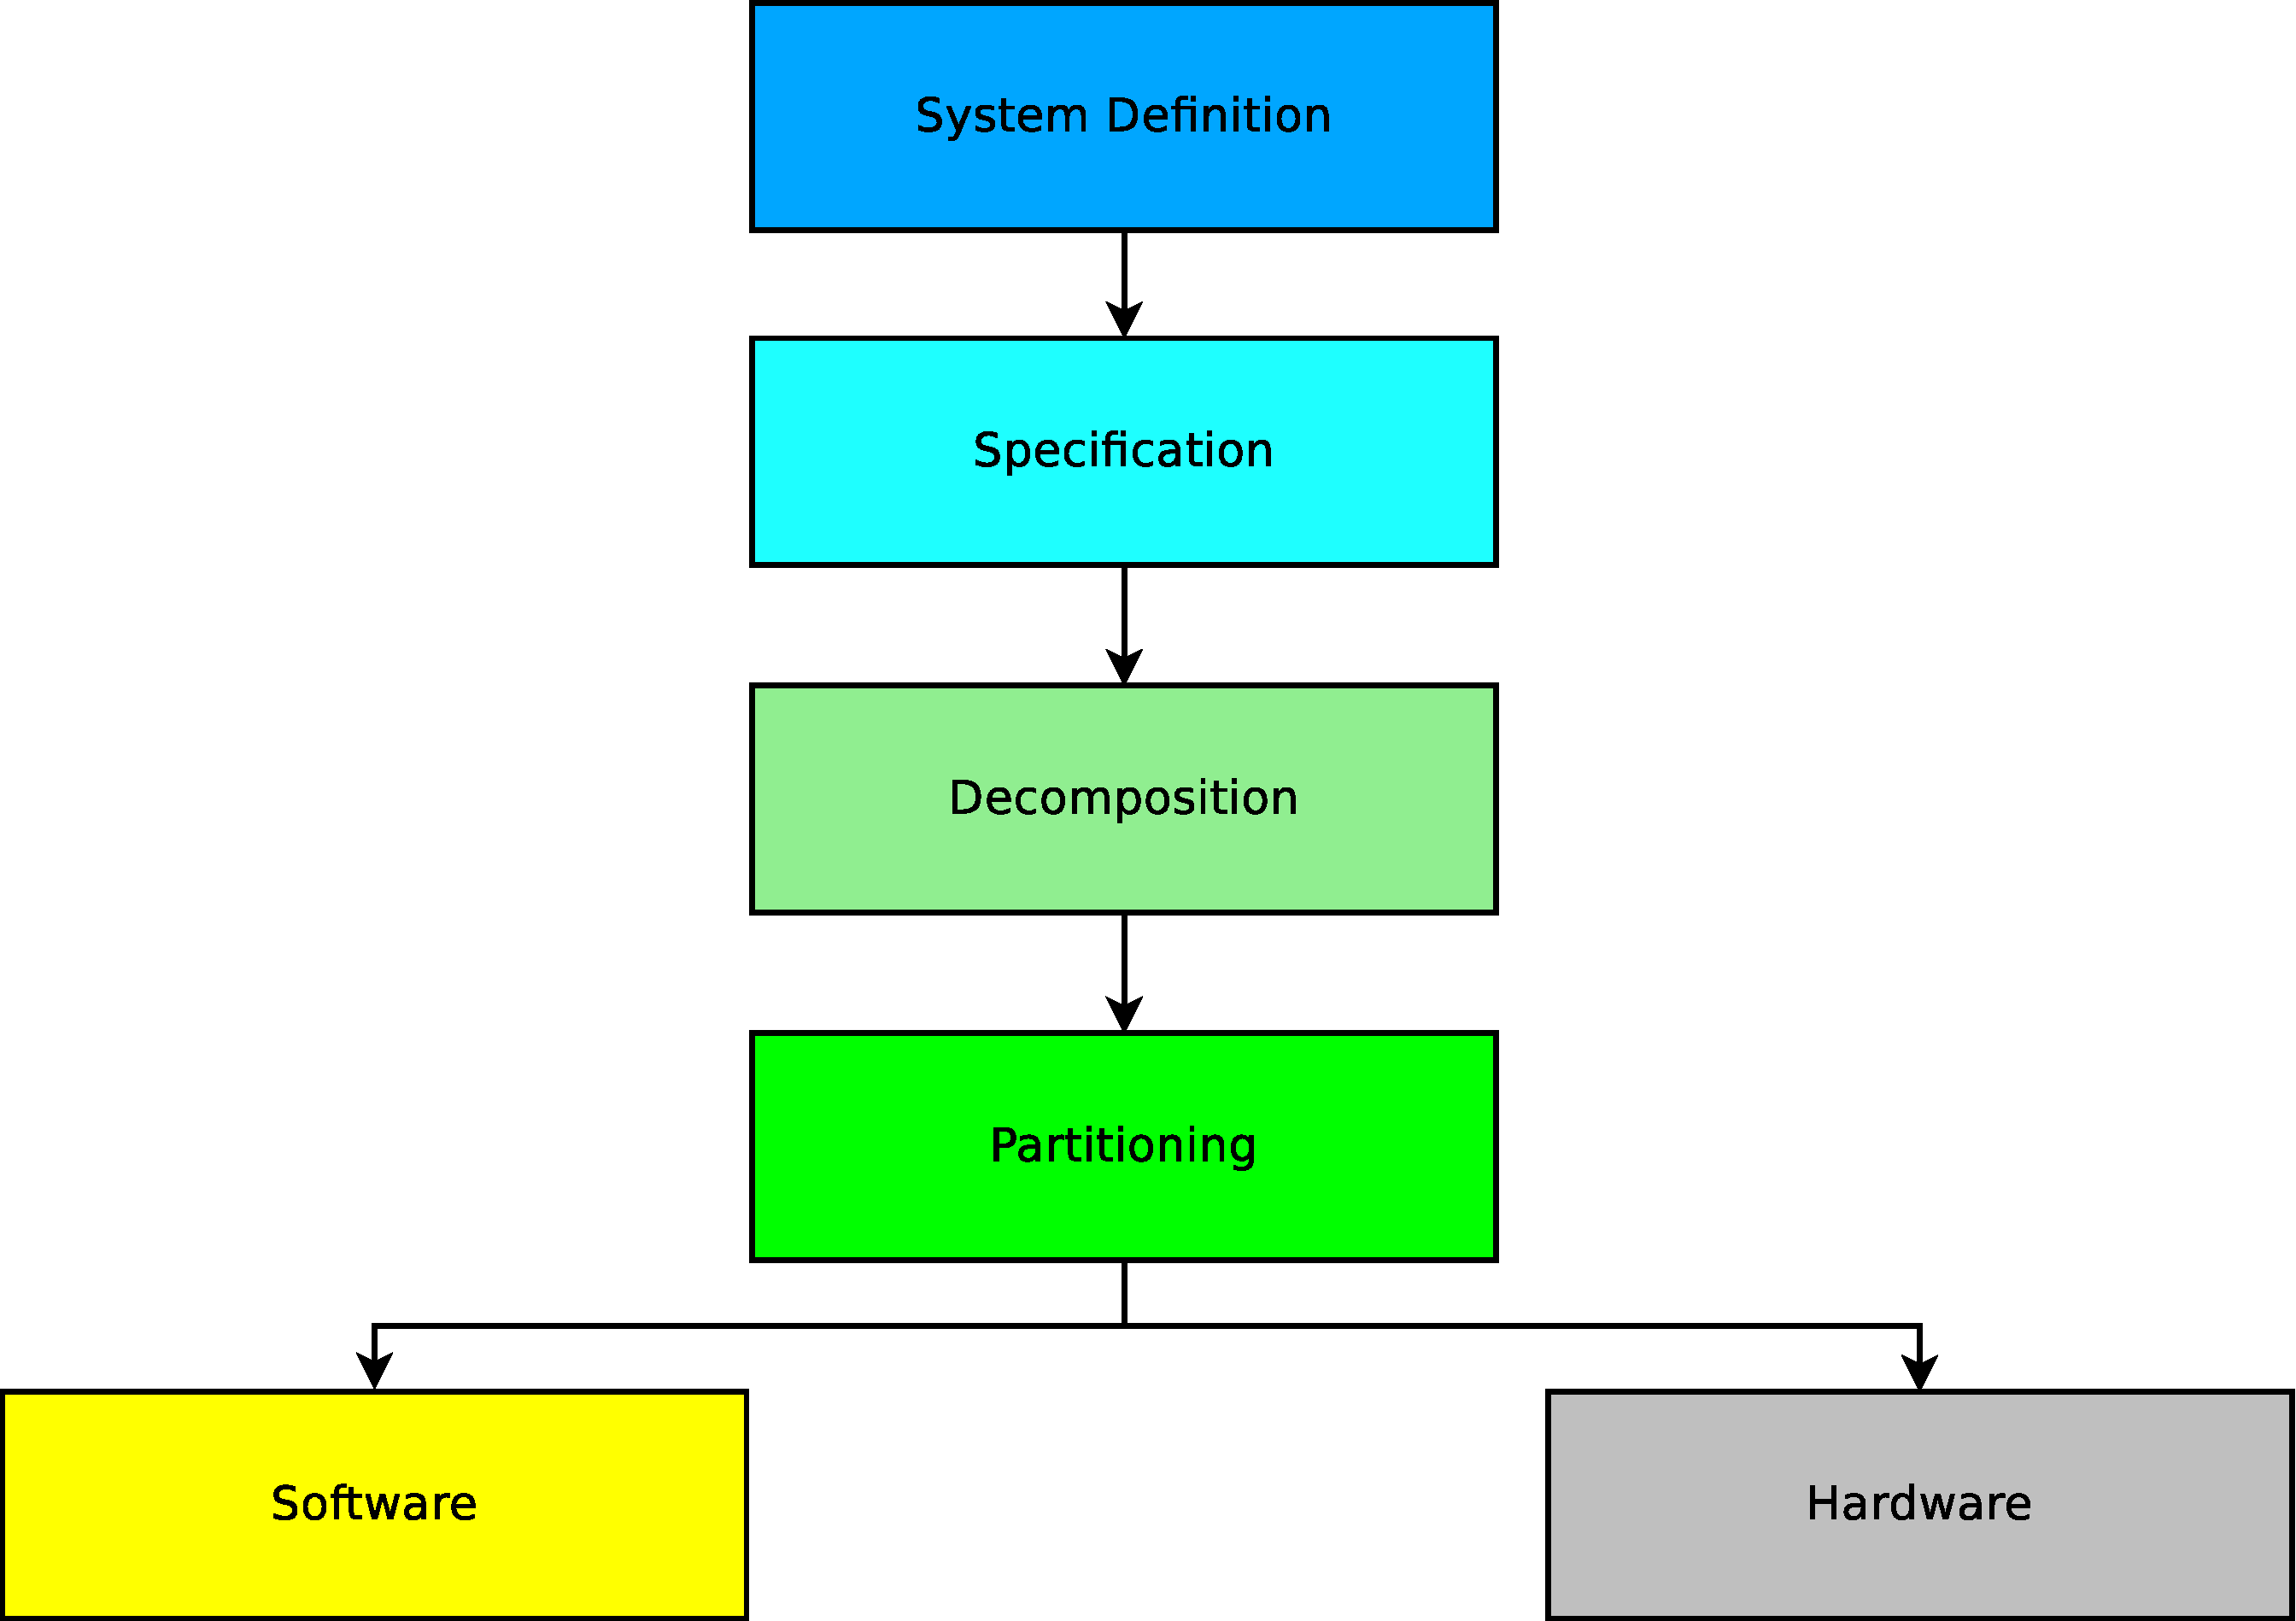
\includegraphics[scale=0.18]{../pictures/flow.pdf}
	      \caption{Design flow \textit{(c.f. Hardware Modelling VO)}.}
	      \label{fig:flow}
	    \end{figure}  
	  If the hardware and software parts should be modified because of, e.g., performance reasons, these two parts must be modified or completely redesigned in order to fit the specifications.
	  This leads to an much higher and probably expensive procedure for the hardware part, thus its design-flow is much longer and every change in the \textit{VHDL/Verilog} code leads to a new compilation, technology-mapping and place and route.
%	  Unless there are other circumstances, the \textit{system definition} and the \textit{specification} steps are part of the project management which have to be done only once.
	\section{Tools}	  
	  \subsection{LegUP}
	  LegUP\footnote{Its current version is 3.0} is an open source high level synthesis tool for fpga based systems from the University of Toronto. 
	  It takes an standart C program as input and implements the hardware fitting part to hardware and the software fitting part to software.
	  LegUP uses an MIPS soft core and uses a standard bus interface for communication between the hardware parts and the processor.  
	  \textbf{Automatic Partitioning? - Yes in a way.}
	  
	  \subsection{Bambu}
	  Bambu\footnote{It can be downloaded at http://panda.dei.polimi.it} is a free framework for the high-level synthesis of complex applications.
	  
	  \subsection{Modelsim}
	  Well known tool for simulation.
	  It also supports SystemC simulation.
	\section{Creators}
	  \subsection{Accellera}
	  Accellera Systems Initiative is a non-profit organization composed of an broad range of members which aims to create system-level standards for the worldwide electronics industry.
	  One of the IEEE\footnote{This standards organization also ratified VHDL, Verilog and SystemVerilog} standards ratified by accellera was IEEE 1666 SystemC.
	  
	\section{Users}
	\subsection{ARM}
	    \begin{figure}[hp]
	      \centering
	      
\includegraphics[scale=0.18]{../pictures/armlogo.jpg}
	      \caption{ARM Ltd.}
	      \label{fig:arm}
	    \end{figure}  
	    ARM (Advanced RISC Machines) Ltd. has an active community\footnote{http://community.arm.com} and there are many informations about tools and IP cores available.
	    SystemC is used by many chip designers and they use the systemC-IP-cores from ARM Ltd. to simulate their designs.
	  \subsection{AMD}
	  
	  \subsection{Intel}
	  
\end{document}
